\section{Paper 1}
    %Begin Table formatting
    \begin{center}
    \begin{tabular}{ | m{5em} | m{25em} |} 
      \hline
      Author(s) Name & Nitin Naik and Paul Jenkins \\ 
      \hline
      Paper Name & Sovrin Network for Decentralized Digital Identity:
    Analysing a Self-Sovereign Identity System Based
    on Distributed Ledger Technology \\ 
      \hline
      Publication Year & 2021 \\ 
      \hline
    \end{tabular}
    \end{center}
    %End Table formatting
    In \cite{9582551}, Self-Sovrin Identity (SSI) model of Identity Management (IDM) has been facilitated by Sovrin Network using Hyperledger Indy. This is governed by Sovrin Foundation.
    Sovrin network consists of ledger layer, agent layer, credential exchange layer and governance layer. It is an open-source identity management system offering decentralized self-sovereign identity, which is built on public permissioned blockchain and governed under the Sovrin Governance Framework (SGF). It employs Indy Plenum consensus protocol which is an improved version of the Redundant Byzantine Fault Tolerance (RBFT) consensus algorithm that offers better security. Sovrin Network offers several important features related to identity and its management such as sovereignty, access control, storage control, recovery management, security, privacy, safeguarding, user-friendliness, governance, and cost-effectiveness; however, it offers only limited support for several important commercial features such as availability, transparency, portability, and interoperability, in establishing it as a global and successful SSI network.It has already adopted several protocols and standards such as DID, VC, DKMS and DID Authentication provided by standard organisations such as the World Wide Web Consortium (W3C), the Organisation for the Advancement of Structured Information Standards (OASIS) and the Decentralized Identity Foundation (DIF). Presently the Sovrin Network offers limited portability, interoperability and scalability.
    It facilitates Decentralised Identifiers (DIDs). Public DIDs are used by issuers that issue proofs and credentials while peer DIDs are used between two parties and are private to them and their relationship. Public DIDs promotes verification of issuer without contacting them. Also Issuer is not required to maintain a highly available verification API / system.
    DIDComm is a protocol that is used for peer to peer communication. 
    \begin{figure}
        
        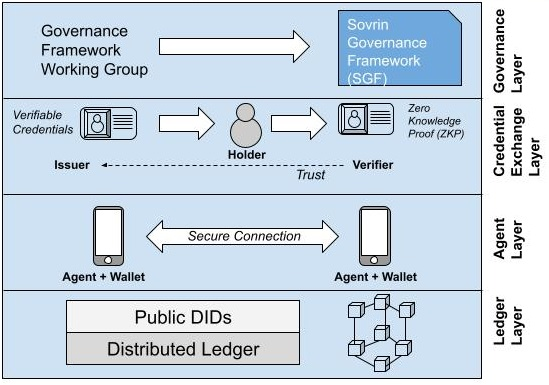
\includegraphics[width=10cm]{images/ArchitectureOfSovrinNetwork.jpg}
        \centering
        \caption{Architecture of Sovrin Network}
        \label{fig:my_label}
    \end{figure}
    
        
    